% ==========================
% GitHub-Friendly LaTeX Report Template (General)
% Minimal deps, clean math, reproducible + public facing
% ==========================
\documentclass[11pt,a4paper]{article}

% ----- Encoding & Fonts -----
\usepackage[T1]{fontenc}
\usepackage[utf8]{inputenc}
\usepackage{lmodern}
\usepackage{microtype}

% ----- Geometry & Spacing -----
\usepackage[margin=1in]{geometry}
\usepackage{setspace}
% \onehalfspacing % uncomment for 1.5 spacing

% ----- Math -----
\usepackage{amsmath, amssymb, amsthm, mathtools, bm}
\usepackage{siunitx}
\sisetup{detect-all}

% ----- Figures & Tables -----
\usepackage{graphicx}
\usepackage{booktabs}
\usepackage{array}
\usepackage{xcolor}
\usepackage{subcaption}
\graphicspath{{figures/}}

% ----- Links & References -----
\usepackage[hidelinks]{hyperref}
\usepackage[capitalise]{cleveref}
\usepackage{csquotes}

% ----- Bibliography -----
% Choose biblatex+biber for modern handling; add references.bib next to this file.
\usepackage[backend=biber,style=authoryear,sorting=nyt,maxbibnames=99]{biblatex}
\addbibresource{references.bib}

% ----- Algorithms (optional) -----
\usepackage{algorithm}
\usepackage{algpseudocode}

% ----- Code listings (safe for GitHub PDF without shell-escape) -----
\usepackage{listings}
\lstset{
  basicstyle=\ttfamily\small,
  frame=single,
  breaklines=true,
  columns=fullflexible,
  showstringspaces=false,
  captionpos=b,
  tabsize=2
}

% ----- Theorem-like Environments -----
\newtheorem{theorem}{Theorem}
\newtheorem{proposition}{Proposition}
\newtheorem{lemma}{Lemma}
\theoremstyle{definition}
\newtheorem{definition}{Definition}
\newtheorem{assumption}{Assumption}
\theoremstyle{remark}
\newtheorem{remark}{Remark}

% ----- Common Macros (customize per project) -----
\newcommand{\E}{\mathbb{E}}
\newcommand{\Var}{\mathrm{Var}}
\newcommand{\Cov}{\mathrm{Cov}}
\newcommand{\Prob}{\mathbb{P}}
\newcommand{\indep}{\perp\!\!\!\perp}
\newcommand{\Pois}{\mathrm{Pois}}
\newcommand{\NB}{\mathrm{NB}}
\newcommand{\Del}{\mathrm{Delaporte}}
\newcommand{\dd}{\,\mathrm{d}}

% ----- Title Block -----
\title{\textbf{From Delaporte to Poisson or Negative Binomial: \\ MH-within-Gibbs Inference and Limits}}
\author{Leonidas Ntrekos \\ \small Email: l.ntrekos@gmail.com \\ \small GitHub:  \href{https://github.com/LNtrekos}{LNtrekos}}
\date{\today}

% ----- Document -----
\begin{document}
\maketitle
\sloppy % fewer overfull lines for GitHub PDF viewers

    % ------------------------------
    \section{Setup}
    This short note presents a reproducible \emph{MH-within-Gibbs} sampler for the Delaporte \emph{Distribution} in R, not so efficient but with nice presentation of the whole methodology. The goal is to estimate (posterior) $(r,p,\lambda)$ from observed (simulated) counts $X_1,\dots,X_n$ and to illustrate (in R) the process where the posterior approaches a Negative Binomial distribution when the Poisson component vanishes or vice versa depending on sample X. The code lives in \texttt{src/delaporte\_sampler.R} figures are auto-generated to \texttt{results/figures/}. 
    
    % ------------------------------
    \section{Model}
    Let $X_i = Y_{1i} + Y_{2i}$ with $Y_{1i} \indep Y_{2i}$ and
    \begin{align*}
    Y_{1i} &\sim \mathcal{NB}(r, p), & \Pr(Y_{1i}=y) &= \frac{\Gamma(y+r)}{\Gamma(r)\,\Gamma(y+1)}\, p^{\,r}\,(1-p)^{\,y}, \\
    Y_{2i} &\sim \mathcal{P}(\lambda), & \Pr(Y_{2i}=z) &= e^{-\lambda}\,\frac{\lambda^{z}}{z!},
    \end{align*}
    where $r>0$, $p\in(0,1)$, $\lambda>0$. This yields the Delaporte distribution for $X_i$.
    
    \paragraph{Priors.}
    We assume a priori independence,
    \[
    \pi(r,p,\lambda)=\pi(r)\,\pi(p)\,\pi(\lambda),
    \]
    and place weakly-informative priors
    \[
    r \sim \mathrm{Gamma}(a_r,b_r), \qquad
    p \sim \mathrm{Beta}(a_p,b_p), \qquad
    \lambda \sim \mathrm{Gamma}(a_\lambda,b_\lambda),
    \]
    where the Gamma is in \emph{rate} parameterization,
    \[
    f(r\mid a,b)=\frac{b^{a}}{\Gamma(a)}\, r^{a-1} e^{-b r}, \qquad r>0,
    \]
    and the Beta density is
    \[
    f(p\mid a,b)=\frac{\Gamma(a+b)}{\Gamma(a)\Gamma(b)}\, p^{a-1}(1-p)^{b-1}, \qquad p\in(0,1).
    \]
    For the examples in this report we take
    \[
    a_r=b_r=0.01,\quad a_p=b_p=1,\quad a_\lambda=b_\lambda=0.01 \ (\text{and} \ n = 100) 
    \]
    but any other weakly-informative choices can be used.
    
    % ------------------------------
    \section{Inference (MH-within-Gibbs)}
    \label{sec:inference}
    Latent counts $Y_{1i}\in\{0,\dots,X_i\}$ are introduced. One sweep consists of:
    \begin{enumerate}
    \item \textbf{Update $\lambda\mid\cdot$.} Given $Y_1$, the full conditional is
    \[
    \lambda\mid\cdot \sim \mathrm{Gamma}\Big(\,\underbrace{\sum_i (X_i - Y_{1i})}_{\text{Poisson totals}} + a_\lambda,\; n + b_\lambda\Big).
    \]
    
    \item \textbf{Update $p\mid\cdot$.} Given $Y_1$ and $r$,
    \[
    p\mid\cdot \sim \mathrm{Beta}\big(\,n r + a_p,\; \sum_i Y_{1i} + b_p\big).
    \]
    
    \item \textbf{Update $r\mid\cdot$ by MH.} With a log-normal random-walk proposal
    $r' \sim \log\mathcal N(\log r, v^2)$, accept with probability $\min\{1,\alpha\}$ where
    \begin{align*}
    \log \alpha
    &=
    \Bigg[
      \sum_{i=1}^n \big(\log\Gamma(Y_{1i}+r') - \log\Gamma(r')\big)
      + n\,r'\log p
      + a_r\log r'
      - b_r\,r'
    \Bigg]
    \\
    &\quad - \Bigg[
      \sum_{i=1}^n \big(\log\Gamma(Y_{1i}+r)\big) - n\log\Gamma(r)
      + n\,r\log p
      + a_r\log r
      - b_r\,r
    \Bigg].
    \end{align*}
    \noindent
    
    \item \textbf{Update $Y_{1i}\mid\cdot$.} For each $i$, enumerate $y=0,\dots,X_i$ and sample with weights proportional to
    \[
    \Pr(Y_{1i}=y\mid\cdot) \propto
    \frac{\Gamma(y+r)}{\Gamma(r)\,\Gamma(y+1)}\, p^{\,r} (1-p)^{\,y}
    \cdot
    \frac{\lambda^{\,X_i-y}}{\Gamma(X_i-y+1)}.
    \]
    
    \paragraph{Stable enumeration for $Y_{1i}$.}
    For each observation $i$ and candidate value $y\in\{0,\ldots,x_i\}$ define the log–weight
    \begin{align*}
    \ell_{iy}
    &= \log\Gamma(y+r) - \log\Gamma(r) - \log\Gamma(y+1)
      \;+\; r\log p \;+\; y\log(1-p) \\
    &\quad +\; (x_i - y)\log \lambda \;-\; \log\Gamma(x_i - y + 1)
      \;-\; \lambda.
    \end{align*}
    The terms $r\log p$ and $-\lambda$ do not depend on $y$ and can be dropped when normalizing.
    To compute probabilities stably, set $m_i=\max_{0\le j\le x_i}\ell_{ij}$ and use
    \[
    \Pr(Y_{1i}=y \mid r,p,\lambda,x_i)
    = \frac{\exp\{\ell_{iy}-m_i\}}{\sum_{j=0}^{x_i}\exp\{\ell_{ij}-m_i\}}
    = \operatorname{softmax}\big(\,\ell_{i0},\ldots,\ell_{ix_i}\,\big)_y .
    \]

    % --- Numerical stability (clamping) ---
    \paragraph{Numerical stability (clamping).}
    To avoid undefined logs when $p$ is arbitrarily close to $0$ or $1$ and when $\lambda$ is close to $0$, we clamp with a tiny $\varepsilon$:
    \[
    \tilde p=\operatorname{clamp}_{01}(p;\varepsilon):=\min\{\max(p,\varepsilon),\,1-\varepsilon\}, 
    \qquad
    \tilde\lambda=\max(\lambda,\varepsilon),
    \]
    with $\varepsilon=10^{-12}$ in our implementation. 
    \end{enumerate}

\section{Chain behaviour across simulated datasets.}
Because $X_i \sim \mathrm{Delaporte}(r,p,\lambda)$ satisfies
\[
\mathbb{E}[X]=\lambda + \underbrace{\frac{r(1-p)}{p}}_{\mu_{\NB}},
\]
many $(r,p,\lambda)$ combinations produce almost the same mean when $n$ is moderate, but with quite different distribution each time.
As a result, the MH-within-Gibbs sampler often exhibits visible ``jumps’’ between two
interpretations of the data:
(i) a \emph{Poisson-like} regime with $r$ small, $p\approx 1$, and $\lambda$ explaining most of
the mean; and
(ii) an \emph{NB-like} regime with larger $r$, moderate $p$, and $\lambda$ near $0$.
    The traces in plot below illustrate these switches; the density panels show the long right tail of $r$
and the concentration of $p$ near the boundary, both typical under weak priors.

\begin{figure}[H]
    \centering
    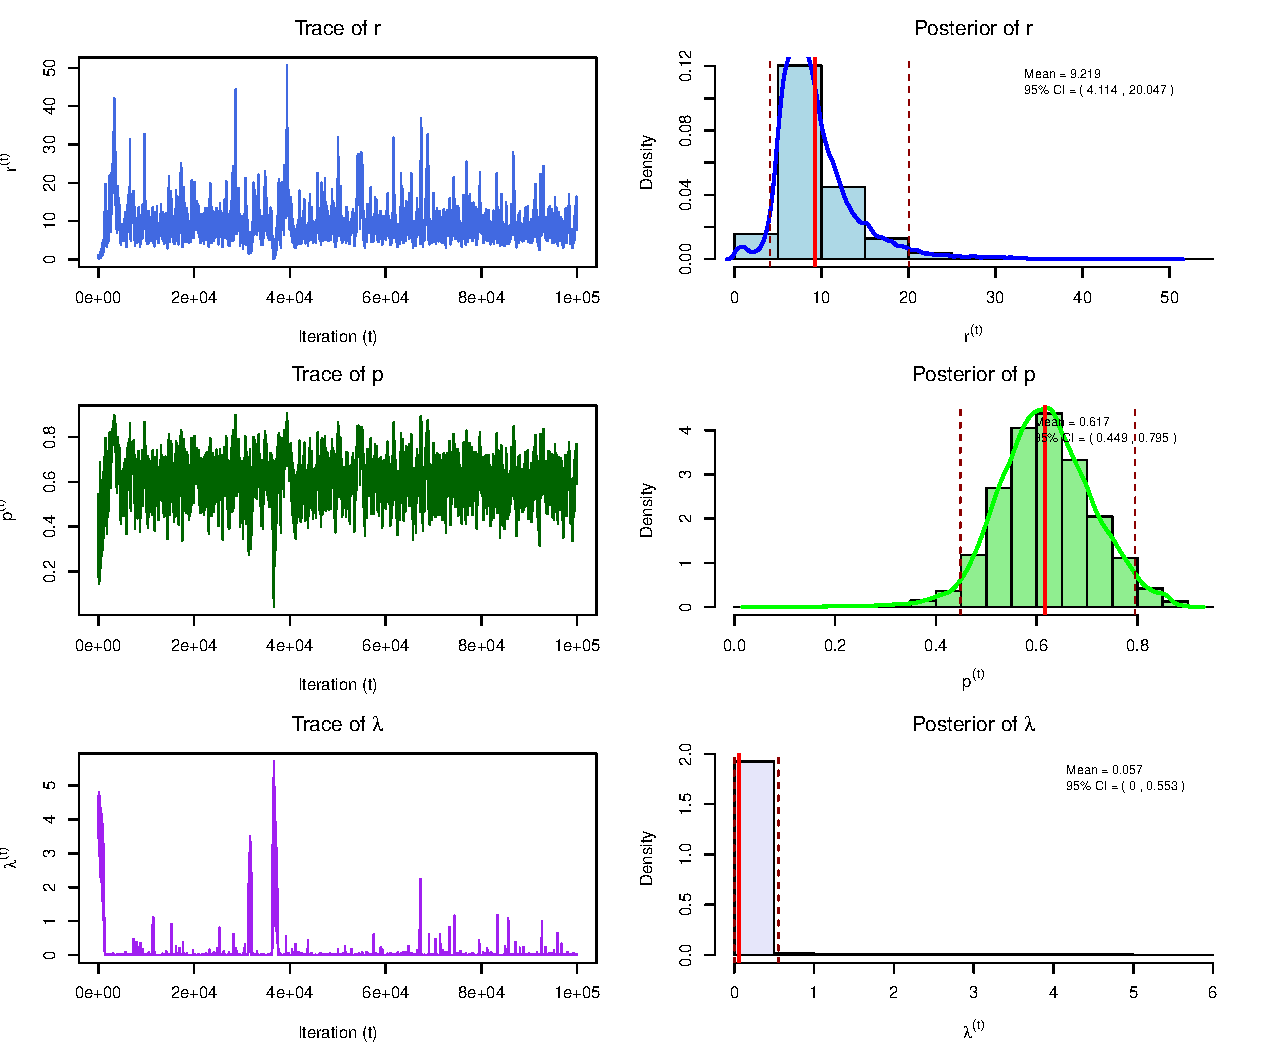
\includegraphics[width=\linewidth]{posterior_plots.pdf}
    \caption{Posterior diagnostics from the repository example: trace plots (left) and marginal posterior densities (right) for $r$, $p$, and $\lambda$; solid lines mark posterior means and dashed lines the 95\% credible intervals. $λ$ is effectively zero (posterior mean 0.057), implying that the Poisson component vanishes in practice; the Delaporte reduces to a near–Negative Binomial fit. }
\end{figure}

\paragraph{Practical notes.}
The observed switching is \emph{posterior multimodality/flatness}, not necessarily non-convergence.
We mitigate numerical issues by clamping $p$ and $\lambda$ (Sec.~\ref{sec:inference}):
$\tilde p=\min\{\max(p,\varepsilon),1-\varepsilon\}$ and $\tilde\lambda=\max(\lambda,\varepsilon)$ with $\varepsilon=10^{-12}$,
and by tuning the $r$ proposal to a $20$--$40\%$ acceptance rate.

Below is the pseudoalgorithm summarising one MH-within-Gibbs sweep using the updates above.


\begin{algorithm}[H]
    \caption{MH-within-Gibbs for the Delaporte model}\label{alg:delaporte-mhwg}
    \begin{algorithmic}[1]
    \Require Data $X_{1:n}$; hyperparameters $(a_r,b_r)$, $(a_p,b_p)$, $(a_\lambda,b_\lambda)$; proposal scale $v$; iterations $T$
    \State Initialize $r^{(0)} > 0$, $p^{(0)} \in (0,1)$, $\lambda^{(0)} > 0$, and $Y_{1i}^{(0)} \in \{0,\dots,X_i\}$ for all $i$
    \For{$t = 1, \dots, T$}
      \State \textbf{Update $\lambda \mid \cdot$}:
      $\displaystyle \lambda^{(t)} \sim \mathrm{Gamma}\!\left(\sum_{i=1}^n (X_i - Y_{1i}^{(t-1)}) + a_\lambda,\; n + b_\lambda\right)$
      \State \textbf{Update $p \mid \cdot$}:
      $\displaystyle p^{(t)} \sim \mathrm{Beta}\!\left(n\,r^{(t-1)} + a_p,\; \sum_{i=1}^n Y_{1i}^{(t-1)} + b_p\right)$
      \State \textbf{Update $r \mid \cdot$ by MH}:
        Propose $r' \sim \log\mathcal N(\log r^{(t-1)}, v^2)$ and accept with probability $\min\{1, e^{\log\alpha}\}$ where
        \begin{align*}
            \log \alpha
        = &
        \Big[\!\sum_i (\log\Gamma(Y_{1i}^{(t-1)}\!+\!r') - \log\Gamma(r')) + n\,r'\log p^{(t)} + a_r \log r' - b_r r'\Big] -\\  & \ \Big[\!\sum_i (\log\Gamma(Y_{1i}^{(t-1)}\!+\!r^{(t-1)}) - \log\Gamma(r^{(t-1)})) + n\,r^{(t-1)}\log p^{(t)} + a_r \log r^{(t-1)} - b_r r^{(t-1)}\Big].
        \end{align*}
        If accepted set $r^{(t)}\gets r'$, else $r^{(t)}\gets r^{(t-1)}$.
      \State \textbf{Update each $Y_{1i} \mid \cdot$ by finite enumeration}:
        For $y=0,\dots,X_i$ compute
        \begin{align*}
            \ell_{iy}
          = & \ \log\Gamma(y+r^{(t)}) - \log\Gamma(r^{(t)}) - \log\Gamma(y+1)
            + r^{(t)}\log p^{(t)} + y\log(1-p^{(t)}) + \\
            & \ \ (X_i - y)\log \lambda^{(t)} - \log\Gamma(X_i - y + 1).
        \end{align*}
        Set $m_i=\max_y \ell_{iy}$ and $w_{iy}=\exp(\ell_{iy}-m_i)$; sample $Y_{1i}^{(t)}$ from $\mathrm{Categorical}(w_{i0},\dots,w_{iX_i})$.
\EndFor
\end{algorithmic}
 \end{algorithm}

 
    
    
    
    


\end{document}

